\documentclass[10pt,a4paper]{article}
\usepackage[margin=17mm]{geometry}
\usepackage{graphicx,booktabs,hyperref}
\pagestyle{empty}
\begin{document}
\noindent{\Large\bfseries Full-call relation instrument: qualification}\\[3pt]
{\small Rust, 27 November 2026. PR \#5251. No measured speedup.}\\[3pt]
{\small $p=2147483647,9007199254740881$; $n=3,4,6$; seed7 LAST-star.}
\paragraph{Result.} The actual root worker and parent transport path pass all 432 fixed-input calls over both launchers, with 432 complete parent proof replays and 1728 deliberate corruptions rejected. Qualification creates no worker performance clocks. All 33 instrument unit functions pass. These are unsigned same-host results, not signed execution attestations. [pcc:unverified]
\begin{center}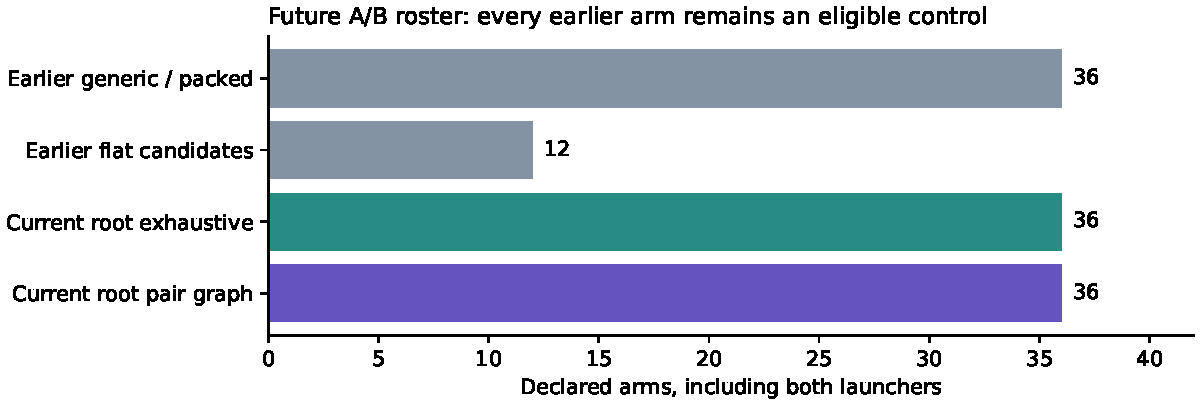
\includegraphics[width=\linewidth]{control-roster.pdf}\end{center}
\noindent The next draft keeps all 48 previous generic/packed/flat arms as eligible controls and adds 36 current-root exhaustive arms. The 36 pair-graph candidates receive identical forms, kernels, launchers and extra readback. The primary is fixed as root-pairgraph-flat-dag-487-native before any performance observations. The design has 168 A/A arms and 120 A/B arms, five rounds and the same six inputs: 8640 future calls, none collected.
\paragraph{Analysis controls.} Two explicitly synthetic cohorts each complete 8640 whole-proof replays. Every clock and monitor flag in these cohorts is invented. Neutral threshold arithmetic is false. Hypothetical 20$\times$ clocks pass threshold arithmetic, while admission remains false. Copied clock-receipt and duplicate-cell sabotage views are both refused with no report. All 51863 neutral-source file hashes remain unchanged. [pcc:unverified]
\begin{center}\begin{tabular}{lrrr}\toprule
Synthetic scenario & Whole proofs & Arithmetic passes & Admission\\\midrule
Neutral &8640 &false &false\\
Hypothetical 20$\times$ &8640 &true &false\\\bottomrule
\end{tabular}\end{center}
\noindent No synthetic number is a host timing, A/A measurement, contention observation or performance result. The analyzer's admission is explicitly false while canonical protocol validation is pending. No 15$\times$ result is established. [pcc:unverified]
\newpage
\noindent{\Large\bfseries Boundary, custody and remaining work}
\begin{center}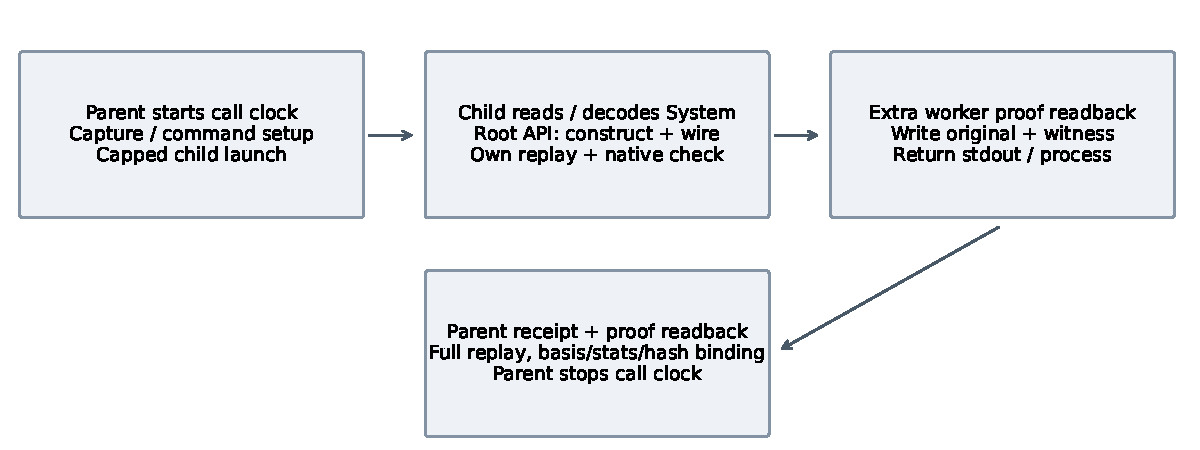
\includegraphics[width=\linewidth]{call-boundary.pdf}\end{center}
\noindent The entire existing parent-call boundary is retained. Case-directory creation and final outcome/report writes remain outside that frozen boundary. Root input decoding, API setup, graph/exhaustive native certification, proof transport and parent full readback remain inside. The coarse root construct phase includes the API's own wire replay; an additional complete worker readback is visible and charged. No root work is amortized or substituted for another proof obligation.
\paragraph{Source custody.} SOURCE\_V2 pins the corrected instrument and unchanged production library. Initial workspace/lock setup and the first compiler failure are retained. System decoding exposes usize exponents; the correction uses fallible u32 conversion. Every registry version/checksum from the prior native lock is preserved. Historical 365/366/372 source and existing evidence are not rewritten. Local workers are copied read-only and hashed before calls. Complete transport, synthetic and corruption-view trees plus immutable workers are archived.
\paragraph{Scope.} Correctness builds use opt0, LTO/debug/incremental off, codegen16, default-features=false, CPU0/jobs1 and one numerical thread. This is not an optimized performance qualification. Prior whole-library libtest allocation failures remain historical failures; this component does not turn them into a whole-library pass. The relation API constructs and certifies a basis; it does not invoke the regular F4 solve. Intrinsic regularity and actual F4 solving degree remain unknown.
\paragraph{CI.} On published head 8d3a59ff303, both native Rust checks and both gate jobs pass. Artifact migration fails PutObject with InvalidAccessKeyId. No key, gate, artifact-store configuration or credential policy is changed. This snapshot is not an all-workflow pass. [pcc:unverified]
\paragraph{Next acceptance.} Original 15$\times$ acceptance is unchanged: prospective full-call timing against the strongest matched controls, both primes, all six fixed cases, repeated/A/A measurements, every proof/failure and published validated evidence. Canonical timing instructions remain encrypted; the separate required-document condition is not waived. Conductor and checkpoint/S3 access have already been waived. No comparative timing or new PCC claim is produced here.
\paragraph{Reproduce.} README and REPRODUCE describe fresh-path builds, no-clock transport, complete synthetic replay and corruption views. Report figures only lay out recorded Rust/configuration values. OUTCOME, source manifests, pre-call worker hashes, raw logs, archives and custody receipts preserve the exact scope.
\end{document}
